% Tackling Climate Change with Machine Learning @ NeurIPS 2026 - Papers track.
% Submission version: no style options, so the style file anonymizes the
% authors and adds review line numbers. Do NOT add [final]; use [preprint] only
% for the arXiv posting after the workshop decision.
%
% Anonymization: the system, platform, and repository names are withheld via
% the \sysname / \platname macros below. Flip them back for the preprint and
% camera-ready.
%
% Figures are generated by research/fairmind-e/analysis/make_figures.py from
% the committed measurement data; regenerate rather than editing the PDFs.

\documentclass{article}

\usepackage[nonatbib]{tackling_climate_workshop_style}

\usepackage[utf8]{inputenc}
\usepackage[T1]{fontenc}
\usepackage{hyperref}
\usepackage{url}
\usepackage{booktabs}
\usepackage{amsfonts}
\usepackage{nicefrac}
\usepackage{microtype}
\usepackage{graphicx}

% Double-blind placeholders. Camera-ready values are in DRAFT.md.
\newcommand{\sysname}{\textsc{EvidenceGate}}
\newcommand{\platname}{an open-source AI governance platform}

\title{Gating AI Deployment on Environmental Evidence Quality}

\author{Anonymous Author(s)}

\begin{document}

\maketitle

\begin{abstract}
Carbon-aware governance proposals gate AI deployment on impact magnitude: a
carbon budget, a readiness level, or a risk rating. None of them asks whether
the carbon number itself can be trusted. We present \sysname, an environmental
governance module deployed inside \platname, that makes measurement provenance
a first-class release criterion: a provenance-derived confidence score crossed
with an impact tier resolves to \emph{go}, \emph{conditional\_go}, or
\emph{no\_go}, and blocks the platform's deployment-approval workflow. In a
measurement study over four workloads, five iterations each, with every
physical run measured by both a software power tracker and an analytic FLOP
model, the release decision changed on \textbf{20 of 20 paired runs} while the
impact tier stayed \emph{low} throughout: the same run was released
unconditionally under one measurement method and held for mitigation under the
other, purely because of how the number was obtained. The two methods disagreed
on magnitude by 123 percent MAPE. A mitigation experiment sharpened the point
in the opposite direction: quantising a fine-tune to \texttt{bfloat16} on a
host with no optimised kernel made it 46 times slower and burned roughly 40
times the energy, so a routine ``we quantised, therefore we cut carbon'' claim
was false by an order of magnitude in the harmful direction. Evidence quality,
not only impact magnitude, decides whether an environmental claim can carry a
release.
\end{abstract}

\section{The gap: a measurement layer with no trust layer}

Regulators and standards bodies are building the measurement layer for AI's
environmental footprint: quantification-methods inventories [1],
sustainability overviews [2], and a G7-commissioned inventory cataloguing
thirteen measurement, monitoring, and reporting initiatives [3]. The EU AI Act
anticipates harmonised standards for ``reporting and documentation processes
to improve AI systems' resource performance'' (Article 40), and
general-purpose AI documentation must state known or estimated energy
consumption (Annex XI) [4]. Yet none of these instruments defines how the
\emph{quality} of an environmental claim should condition a deployment
decision.

Recent governance research gates on magnitude. Carbon-aware governance gates
embed carbon budgets in governance layers, recording provenance only in audit
logs [5]. Sustainability-pyramid frameworks gate on readiness levels [6], and
risk-management integrations treat AI carbon as a risk dimension in banking
frameworks [7]. Meanwhile measurement research has established that
reliability varies sharply with disclosure: metadata-completeness tiers across
5{,}227 public models span roughly $1.2\times$ to $2\times$ estimation error
[8], and spend-based fallbacks in tiered Scope~3 accounting overestimate by
10--40$\times$ [9]. Adjacent work has begun to act on estimate trust, through
conformal calibration inside a carbon budget gate [10] and confidence-gated
filtering of industrial emissions predictions [11]. The two literatures have
not been connected: a system can sit comfortably under its carbon budget while
its carbon number is untrustworthy, and every published gate would pass it.

Our claim is narrow and, to our knowledge, unheld: environmental \emph{evidence
quality}, not only impact magnitude, should gate AI deployment. The
intellectual ancestry is the data-quality tradition in life-cycle assessment,
where pedigree matrices and data quality indicators grade the provenance of an
inventory figure [12], and the NUSAP uncertainty pedigree [13]. Recent work
recommends indicator-style disclosure for AI-assisted product footprinting but
proposes no score, no thresholds, and no gate [14]. We invert that tradition:
where it assesses AI that produces carbon numbers, we score carbon numbers to
gate the AI.

\section{Mechanism}

\paragraph{Provenance classes and confidence.} Every assessment declares its
measurement source, normalized to one of five provenance classes with bounded
confidence ranges: \emph{measured} (hardware telemetry; 0.85--1.00),
\emph{tool\_estimated} (software power trackers; 0.60--0.85),
\emph{vendor\_reported} (cloud-provider figures; 0.40--0.60), \emph{manual}
(analytic FLOP estimates; 0.20--0.40), and \emph{unknown} (0.0). A
caller-supplied score is honoured but never allowed to exceed its provenance
cap, and unknown provenance forces 0.0 regardless of any claimed score.
Provenance is categorical and reported separately from quantified uncertainty,
so a precise-looking number cannot launder a weak source.

\paragraph{Tiers and the decision matrix.} Metrics map to low, medium, or high
impact per lifecycle phase, using location-based carbon so market instruments
cannot lower a gate outcome. Confidence bands (measured $\geq 0.70$; estimated
0.35--0.69; unknown $< 0.35$) cross with impact tiers into the matrix shown in
Figure~\ref{fig:main}(b). Confidence 0.0 short-circuits to \emph{no\_go} before
matrix lookup: an undisclosed claim never passes. A \emph{conditional\_go}
cannot be approved until it carries a dated, owned mitigation or an explicit
exception with owner, expiry, and rationale, which makes reviewer overrides
auditable rather than informal. Six controls (ENV-1 to ENV-6: boundary, energy
accounting, dual location and market carbon, per-functional-unit efficiency,
evidence confidence with disclosed uncertainty, and mitigation or exception)
define coverage. Disclosed offsets are recorded but never subtracted from
emissions and never improve any gate output.

\section{Implementation}

\sysname{} ships inside \platname, not as a standalone proposal. The decision
engine is a framework-agnostic Python package with 57 unit tests covering every
matrix cell, band boundary, provenance cap, and the undisclosed-evidence
short-circuit. Assessments persist as versioned governance evidence, and a
release gate hooks the platform's existing deployment-approval workflow,
returning HTTP 409 with the blocking reason when the latest assessment is
\emph{no\_go} or an unmitigated \emph{conditional\_go}. Reviewers get an
interface showing the matrix position, control coverage, mitigation tracker,
and version trail, and disclosures export in a format shaped to the European
sustainability reporting standard for climate change [15].

On a 14-case hand-labelled fixture set spanning all matrix cells, mitigation
states, exception paths, and offset disclosures, the full mechanism reproduces
14/14 expected labels, while ablations degrade sharply: a carbon-only gate
manages 7/14, a generic sustainability score 6/14, and no environmental gate
3/14, with removing only the exception path or the mitigation review costing
one to three cases each. The authors wrote both the fixtures and the engine,
so this is a consistency illustration showing the confidence dimension is
load-bearing, not an empirical validation. That is what the next section is
for.

\section{Measurement study: provenance decided the release}

\begin{figure}[t]
  \centering
  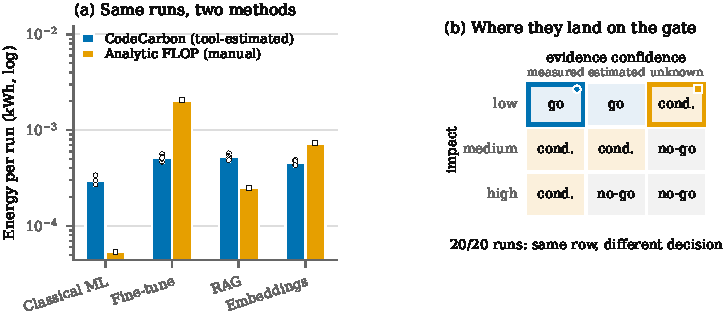
\includegraphics[width=\linewidth]{figures/fig1_provenance_decides.pdf}
  \caption{Four workloads, five iterations each, every physical run measured
  twice. (a) The two methods disagree on energy by 123 percent MAPE, and not
  in a consistent direction. (b) The production decision matrix; outlined
  cells mark where the study's runs landed. Both methods put every run in the
  same \emph{low} impact row, so magnitude drove nothing: the column moved
  because provenance moved, and with it the release decision.}
  \label{fig:main}
\end{figure}

Four workloads (classical ML training, transformer fine-tune, RAG inference,
batch embeddings) ran five iterations each on a single host. Every physical run
was measured three ways: a software power tracker
(\emph{tool\_estimated}), operator-filled cloud billing
(\emph{vendor\_reported}), and a documented analytic FLOP model
(\emph{manual}). The harness never fabricates: cloud billing lags execution by
hours to days, so its 20 records are explicit unavailable entries with a stated
reason rather than imputed numbers. All runs were replayed through the
production engine, not a reimplementation.

\textbf{The decision changed on 20 of 20 paired runs.} The power tracker mapped
to \emph{tool\_estimated}, confidence 0.72, the \emph{measured} band, and
\emph{go}; the FLOP model mapped to \emph{manual}, confidence 0.30, the
\emph{unknown} band, and \emph{conditional\_go}. The impact tier was
\emph{low} in every case (Figure~\ref{fig:main}(b)), so nothing about the
magnitude produced the difference. The same physical run was released
unconditionally under one measurement method and held for mitigation under the
other, purely because of how the number was obtained. A carbon-budget gate or
a readiness-level gate sees \emph{low} impact in both columns and passes both.

Method agreement is poor in its own right: MAPE 122.6 percent with the tracker
as reference and 169.1 percent with the FLOP model as reference, ranging from
52 to 298 percent by workload, with Bland-Altman limits of agreement spanning
$-1.15{\times}10^{-3}$ to $1.79{\times}10^{-3}$~kWh.

\begin{figure}[t]
  \centering
  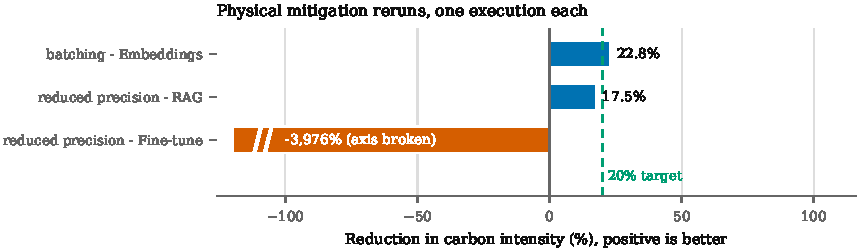
\includegraphics[width=\linewidth]{figures/fig2_mitigations.pdf}
  \caption{Mitigation outcomes. Ten of eleven pairs reduced carbon intensity,
  four of them past the 20 percent target. One inverted the mean: quantising
  the fine-tune from \texttt{float32} to \texttt{bfloat16} on a host with no
  optimised kernel took it from 62.7\,s to 2887.6\,s and burned roughly 40
  times the energy. That bar is truncated and labelled with its true value.}
  \label{fig:mitigations}
\end{figure}

\paragraph{Mitigations, and a claim that was false in the harmful direction.}
Four interventions were measured as pre/post pairs
(Figure~\ref{fig:mitigations}). The pre-registered test that mitigations
reduce intensity by more than 20 percent is \textbf{not supported}: paired
$t = -0.859$, $p = 0.410$ over 11 pairs, mean reduction $-311$ percent. Ten of
eleven pairs did reduce, with a median of 33.9 percent. One pair inverted the
mean: quantising the fine-tune from \texttt{float32} to \texttt{bfloat16} made
it 46 times slower, because the host had no optimised reduced-precision kernel,
and burned roughly 40 times the energy. Reporting only the median, or dropping
the outlier, would be cherry-picking, so the pre-registered result stands as
computed.

This is the mitigation analogue of the paper's argument. ``We quantised the
model, therefore we cut carbon'' is a routine and entirely plausible claim; on
this hardware it was false by more than an order of magnitude, in the harmful
direction. A gate that accepts asserted mitigations would have recorded a
reduction that never happened, which is why ENV-6 requires the mitigation to be
documented and re-measured rather than declared.

\paragraph{Expert panel (registered, in progress).} Twelve engine-validated
profiles covering all nine matrix cells are rated by 15 reviewers across
governance, ML engineering, and sustainability roles under a two-arm
counterbalanced design (baseline: raw measurements only; module: full
\sysname{} output), testing whether displayed confidence correlates with
conservatism, whether the module arm raises ENV control coverage, and whether
the matrix improves inter-rater agreement. Instrument and analysis are
implemented; we seek critique of the baseline arm before collection closes.

\section{Pathway to climate impact}

Environmental reporting for AI is moving from voluntary to mandatory, but
mandatory reporting only reduces emissions if the reported numbers are
trustworthy enough to act on. Our measurement study shows the gap is not
hypothetical: two standard methods applied to the same run disagreed by more
than 100 percent and implied opposite release decisions, and a textbook
efficiency intervention increased emissions fortyfold while a
declaration-based gate would have logged it as a reduction. Making evidence
quality a release criterion changes the incentive directly: a team that cannot
substantiate its number cannot ship unconditionally, so measurement effort
becomes the cheapest path to approval rather than an unrewarded cost. This is
a leverage point rather than direct abatement: it does not itself cut
emissions, it makes the reductions others report verifiable and therefore
actionable. The near-term channel is regulatory: Article 40's harmonised
standards for resource-performance reporting do not yet exist [4, 16], and a
provenance-scored, platform-integrated gate is a concrete, testable proposal
for what they could require.

\paragraph{Limitations.} The study host exposes no hardware energy counters, so
the tracker fell back to load-based estimation: this study compares an estimate
against an estimate and never claims the \emph{measured} provenance class.
These are benchmark workloads, so only the low-impact row is exercised and the
provisional thresholds cannot be recalibrated from this data. The FLOP model
uses placeholder efficiency constants, and the panel targets 15 raters, sized
for feasibility rather than power. Code, data, and figure scripts are public.

\begin{ack}
Withheld for double-blind review.
\end{ack}

\section*{References}

\small

[1] CEN/CLC/TR 18145:2025. {\it Environmentally sustainable artificial
intelligence: quantification methods inventory.} 2025.

[2] ISO/IEC TR 20226:2025. {\it Artificial intelligence: environmental
sustainability aspects.} 2025.

[3] G7 French Presidency (2026) {\it Overview of initiatives for the
measurement and monitoring of energy and resource use of AI models.} May 2026.

[4] Regulation (EU) 2024/1689 (Artificial Intelligence Act), Article 40 and
Annex XI \S1(2d). 2024.

[5] Carbon-aware governance gates: embedding carbon budgets, energy provenance,
and sustainability-aware validation in governance layers. arXiv:2602.19718v2,
2026.

[6] G-TRACE: an AI sustainability pyramid for carbon-aware governance
readiness. arXiv:2511.04776v3, 2026.

[7] Tkachenko, N.\ (2025) Sustainable integration of frontier AI in banking.
{\it Journal of Financial Compliance.}

[8] Hugging Carbon: estimation reliability tiers for the carbon footprint of
5{,}227 public models. arXiv:2605.01549v2, 2026.

[9] A four-tier Scope 3 methodology for AI inference under CSRD.
arXiv:2606.10660, 2026.

[10] Green SARC: predictive cost and carbon governance for agentic AI with
split-conformal calibration. arXiv:2606.15954, 2026.

[11] Trust-aware predictive emissions monitoring: confidence-gated filtering of
industrial emissions estimates. arXiv:2606.06156, 2026.

[12] Weidema, B.P.\ \& Wesn\ae s, M.S.\ (1996) Data quality management for life
cycle inventories: an example of using data quality indicators. {\it Journal of
Cleaner Production} {\bf 4}(3--4):167--174.

[13] Funtowicz, S.O.\ \& Ravetz, J.R.\ (1990) {\it Uncertainty and Quality in
Science for Policy.} Dordrecht: Kluwer.

[14] Criteria for credible AI-assisted carbon footprinting systems.
arXiv:2509.00240, 2025.

[15] Directive (EU) 2022/2464 (Corporate Sustainability Reporting Directive)
and ESRS E1, Climate change. 2023.

[16] Regulating the environmental footprint of AI: the regulatory landscape.
arXiv:2603.00068, 2026.

\end{document}
